\section{Monte Carlo Generators}
\label{section: mc generators}

Monte Carlo (MC) generators are computational software used to simulate high energy processes. They use the principles of random sampling to emulate quantum mechanical phenomena together with the Standard Model and phenomenological models to describe particle interactions. %Since these processes are computed this gives physicists a full and exclusive modelling of high energy processes.

%Event generation is composed of two phases. The first is the generator stage which simulates the interaction between two initial particles (generally beam particles such as the proton-proton beams at the LHC) and the resulting particles from the parton interaction including their subsequent decays and the remnants (beam remnants in the case of LHC interactions). The second stage simulates the interactions between the particles produced in the initial stage and the components of the detector. This includes the simulation of particles which are produced from interactions with detector material as well as electromagnetic fields present in the detector. Furthermore the electronic signals from the detector components are also simulated. In the case of a perfect detector the result of the detector simulation would yield the particles produced in the generator stage, though in practise this is not the case.

MC generators are important for many aspects of high energy physics. They enable physicists to develop an understanding of how physics models translate to real world experiments bridging between the theoretical and experimental aspects of high energy physics. MC generators provide physicists insight into the frequency of specific types of events as well as the angular distribution of the resultant particles. This enables physicists to estimate the signal to background ratios of specific processes and provide insight into which regions of phase space provide the greatest level of sensitivity for a given process. Understanding the distribution of the resultant particles from a given type of interaction enables highly specialist detector design optimised for sensitivity to a given process.

MC generators are extremely sophisticated programs due to the complexity of high energy process. This process is simplified by factorising the process into several steps. First a hard process is simulated with associated initial state radiation followed by the hadronisation process and final state radiation as well as beam remnants. These components are discussed in the following sections and are visualised in figure \ref{fig: event schematic}.

\begin{figure}[h]
	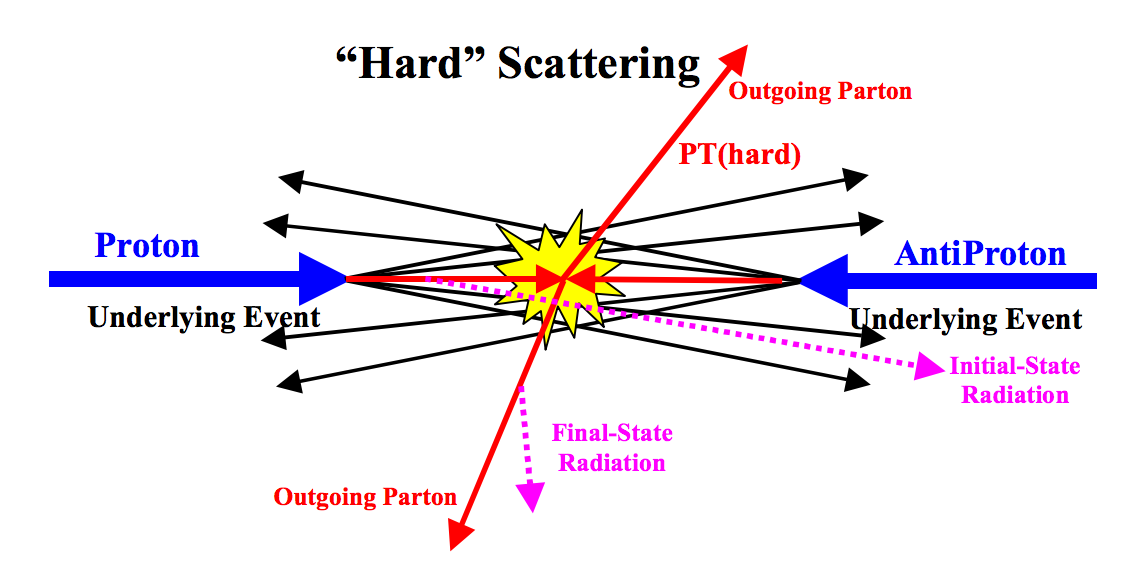
\includegraphics[width=\textwidth]{/Users/admin/projects/phd/thesis/latex/Chapters/theory/mc_generators/images/event_schematic.png}
	\caption{An event schematic demonstrating the aspects of the interaction \cite{Field:2002vt}}
	\label{fig: event schematic}
\end{figure}

%MC generators are extremely sophisticated programs though complexity of high energy processes rivals this. In order to make the process of event generation simpler the process is decomposed into components simplifying the problem via the principle of factorisation. Several of these components are discussed in the following sections.

%\subsection{Physics Model}
\subsection{The Hard Process}

The hard process is described by the parton interaction with the highest momentum transfer, it characterises the properties of the event such as the distribution of particles in the system and their energies. In general, experimentalists are interested in events involving a particular hard process, such as the production of exotic flavoured states, e.g.

\begin{equation}
	\mathrm{gg} \rightarrow \mathrm{c\bar{c}}
\end{equation}

describing the process of gluon fusion forming a charm quark-antiquark pair.

The hard process is the first stage of a MC event simulation, next a backwards time evolution is performed on the initiator partons to describe the system before the interaction. In the proton-proton event case this corresponds to the state of the incoming proton pairs. Similarly a forward time evolution is applied to the outgoing partons of the interaction to describe the final state of the system.

The forward evolution is divided into two phases, the first stage describes the radiation of quarks and gluons from the outgoing partons as a series of parton branchings evolving the system from a state with a low number of high momentum partons to a state with a high number of low momentum partons (parton shower \ref{section: parton shower}). This process describes the branchings using perturbative calculations down to a momentum threshold where perturbative methods are no longer applicable. Similarly an upper momentum threshold exists; partons with a momentum greater than this threshold are assigned to the hard process of the event.

The second phase takes the output of the parton shower and evolves it into a system of colourless hadrons using non-perturbative phenomenological models via the process of hadronisation (section \ref{section: hadronisation}). 

%
%\begin{equation*}
%	Q >> \Lambda
%\end{equation*}
%
%where $Q$ is the momentum transfer in the process and $\Lambda$ is the QCD scale ($217^{+25}_{-23}$ MeV), the strong coupling constant for these momentums is small allowing the cross-section for these processes to be calculated perturbatively.

\subsection{Initial and Final State Radiation}
\label{section: parton shower}

Initial state radiation is composed of partons that are emitted from the  beam particles. In the case of proton beams this is modelled as virtual particles being exchanged between the quark constituents; these virtual particles primarily consist of gluons which may further radiate pairs of gluons creating a complicated state of the proton. Similarly final state radiation consists of a myriad of partons but in this case the partons originate from the out-going partons of the hard scatter and initial state radiation.

The probability for branching to occur is generally calculated in one of two ways, either with a matrix element calculated from Feynman diagrams or with the parton shower model. The parton shower model is a simplified version of the matrix element approach with approximations including a simplification of kinematics, interference and helicity structure. Though the matrix element calculations are truer to the theory of QCD, in practice the matrix elements are more difficult to calculate - especially at higher orders. The two approaches are complementary to one another and which approach is used is based on the particular situation. In general the parton shower is chosen as the first place to start due to its flexibility and simplicity whilst for precision measurements the matrix element approach is favoured.

\subsubsection*{Parton Showers}
The parton shower is made up of branchings of the form $a \rightarrow bc$, e.g for quark-gluon radiation this is, 

\begin{equation*}
	q \rightarrow qg
\end{equation*}

Each of the partons in a shower are characterised by its virtuality scale $Q^2$ which gives an approximate sense of its time ordering in the shower, classically it is defined as the invariant mass of the parton; under this definition a system with a low number of high mass partons evolving into a high number of low mass partons will decrease in the virtuality scale as more and more branchings occur. The $Q^2$ variable may also be described by other variables such as its transverse momentum which similarly decreases with the number of branchings. A maximum virtuality scale $Q_{\mathrm{max}}$ distinguishes partons that are involved in the hard process from those in the parton shower, also a minimum virtuality scale $Q_0$ sets the scale at which non-perturbative effects become significant.

Partons with $m^2 < 0$  and $m^2 \ge 0$ are described as space- and time-like respectively. 

\subsubsection*{Initial State Radiation (ISR)}
For initial state radiation the virtuality scale is typically associated to the mass of the parton given by the equation,

\begin{equation}
	Q^2 = -m^2 = -(E^2 - p^2)
\end{equation}

The branching evolution of initial state radiation is described by increasing values of the virtuality scale $Q^2$, this corresponds to a high energy parton from a beam particle emitting partons with increasing virtuality and momentum i.e. the branching partons become more space-like. The branching continues until there are enough partons with $Q^2 \ge Q^2_{\mathrm{max}}$ to initiate the hard process; thus limiting the virtuality of the system, for example, the virtuality of the partons in the process $q\bar{q} \rightarrow Z^0$ have a virtuality cut off of the order of the $2m_{Z^0}$.

In order to generate an event with a particular hard process the shower algorithm first sets the longitudinal momentums $x_1$ and $x_2$ of the incoming partons to that required by the hard process using the parton distribution function. A backward time evolution is then applied to the partons, gaining energy with each emission and decreasing in virtuality until it is compatible with a shower initiating parton in the proton.

\subsubsection*{Final State Radiation (FSR)}
For final state radiation the initiating shower parton originates from the outgoing partons of the hard interaction via time-like partons. The virtuality scale for partons is typically defined by either its invariant mass or transverse momentum.

\begin{equation}
	Q^2 = m^2
\end{equation}
or
\begin{equation}
	Q^2 = p_\perp^2
\end{equation}

note the change in sign in the mass ordering relative to the ISR. The final state evolves with a decreasing virtuality scale - becoming more time-like. Starting from an outgoing parton from the hard process the branching results in partons with lower mass or transverse momentum depending on the choice of ordering parameter. The minimum virtuality of a parton is set by $Q_0$, partons which cannot branch further due to this cutoff are then used as input for the hadronisation process.

%There are several options for the evolution parameter for final final state radiation. Most common are the invariant mass $m$ and the transverse momentum of the parton $p_\perp$. In contrast to initial state radiation the evolution parameter generally decreases with more branchings, 

%Final state radiation consists of partons radiated from the outgoing partons of the hard process. The cascade of partons are modelled by the DGLAP equations and works downwards to lower momentum scales to a point where perturbation theory breaks down. At this point the partons are evolved to colourless hadrons via the process of hadronization.
\subsection{Hadronisation}
\label{section: hadronisation}
\subsection{The Underlying Event}
\label{section: underlying event}

The underlying event is any other activity in an event that accompanies a hard process, it contains contributions from the beam remnants - the left over proton fragments after the hard scatter - multiple parton interactions and initial and final state radiation. The hard scatter consists of the two outgoing jets, the initial state radiation leading to the hard process and the particles originating from the hard final state radiation.

The beam remnants are particles that evolves from the remainder constituents of the beam particle that do not take part in the hard process. These may be colour connected to the hard process due to colour confinement e.g. for a proton-proton interaction, a proton that initiates a hard process via a quark initiator will have remaining constituents that form a colour triplet. The colour connections are later resolved during the hadronisation process which ensures the final state of the interaction is composed of colour singlet hadrons. 

%Pythia: Highly developed multiple interaction model
%HERWIG: A MPI model is built into Herwig++ but a separate module (JIMMY) has to be interfaced to the Fortran version

%Lorentz contraction of highly boosted beam particles in result in disc like shapes in the laboratory rest frame. Interacting partons from the beam particles are extremely localised such that the parton shower and subsequent hadronisation are also. An overlap between the other partons in the beam particles giving rise to the potential of Multiple Parton Interactions (MPI) each with their own associated parton shower and hadronization. The additional interactions in multiple parton interactions are dominated by soft interactions though contributions exists from hard and semi-hard interactions. 

% and have been shown to have a significant effect on the particle multiplicity of the event.


% Beam remnant: Particles which do not take an "active" part in the initial-state radiation or hard-scattering process.
% 	Is colour connected to the primary 
% Multiple interactions: When more than one parton from each beam particle have "significant" interactions. in a fraction of events these additional scatterings maybe hard or semi-hard, but mostly they are soft in comparison to the hard process
% 	Important to model the impact parameter structure of hadron-hadron collisions
%	Impact parameter: Measure of how much overlap there is between hadrons
%		If it is small there is a high probability of multiple interactions
%		if it is small there is a high probability of a hard scatter
%		thus if it is small there is on average a higher amount of underlying event activity
%		if it is large there is a small probability of multiple interactions
% Primordial $k_\perp$: Transverse momentum of the shower initiating parton - takes into account the motion of quarks inside the original hadron.
% Underlying event: Arises from collisions between partons in the incoming hadrons that do not directly participate in the hard subprocess
% 	Everything except the hard radiation from the matrix element in the hard process for a single particle collision
% 	Minimum bias data - not identical but still related. Used to study correlations...

% MPI
%The most common hard subprocess at a high-energy hadron collider, such as the LHC, is elastic gluon-gluon scattering, $gg \rightarrow gg$ . The leading-order differential cross section for this subprocess diverges at zero momentum transfer, due to the exchange of a massless virtual gluon. This indicates that there are many interactions between beam particles though of a soft nature. 

%Multiple parton interactions is a term used to describe a proton-proton collision in which more than one parton from each of the protons are involved in an interaction. In general a proton-proton interaction is described by its primary interaction i.e. the parton interaction at the highest interaction scale, relative to this additional interactions are soft scale interactions due to an asymptotically decreasing cross-section with the interaction scale. However the probability of additional interactions that are hard or semi-hard is significant and has considerable effects on distributions such as the particle multiplicity.

% Why is it important
%A rather mundane reason for this is that if two pairs of partons collide in a single proton-proton collision, this can lead to some very peculiar-looking events. Two "standard" collisions can gang up and look very non-standard, possibly leading you to think you have found some physics beyond the Standard Model. (Probably supersymmetry.) So if you want to claim this, you need some understanding of the probability of multiparton interactions occurring in a single proton-proton collision.
%
%But on top of that, the issue of how a strongly interacting quantum field theory gives rise to the proton, an ultra-stable bound state with a lifetime longer than the age of the universe, present in the heart of every atom of matter, is an exciting open question. It's a problem being tackled from several experimental, theoretical and computational directions. I think understanding correlations between partons in high energy collisions will make an important contribution to this.
\subsection{Multiple Parton Interactions (MPIs)}
%Multiple parton interactions is a term used to describe a proton-proton collision in which more than one parton from each of the protons are involved in an interaction. In general a proton-proton interaction is described by its primary interaction i.e. the parton interaction at the highest interaction scale, relative to this additional interactions are soft scale interactions due to an asymptotically decreasing cross-section with the interaction scale. Though the probability of hard or semi-hard additional interactions are smaller than for soft interactions at higher energies this increases due to the ability of partons to resolve partons in the proton with lower longitudinal momentum fraction $x$.

Multiple parton interactions is a term used to describe a proton-proton collision in which there is more than one hard scatter between the constituent partons. Observations of MPI effects can be seen in data from hadron collisions at the Intersecting Storage Rings (ISR) at CERN \cite{Akesson:1986iv} and the Fermilab Tevatron collider \cite{Abe:1997bp} \cite{Drees:1996rw} \cite{Abazov:2009gc}. Soft MPI effects have been observed in proton-proton collisions at Collider Detector Fermilab (CDF) \cite{Acosta:2004wqa} \cite{Aaltonen:2010rm} and CMS \cite{Khachatryan:2010pv}.

%The evidence for MPI comes from high pT events observed in hadron collisions at the ISR at CERN [1] and later
%at the Fermilab Tevatron collider[2, 3, 4]. At lower pT, underlying event (UE) observables have been measured in pp
%collisions in dijet and Drell-Yan events at CDF in Run I [5] and Run II [6] at centre-of-mass energies of p
%s = 1:8 TeV
%and 1:96 TeV respectively, and in pp collisions at p
%s = 900 GeV in a detector-specic study by CMS [7].
%At small transverse momentum MPI have been shown to be necessary for the successful description of th

It is important to understand MPI for several reasons. In the case of rare and exotic physics, two simultaneous non-exotic hard interactions may lead to non-standard looking events, it follows that in order to identify rare interactions and claim a discovery, one must have some understanding of the effects from MPI. Furthermore understanding MPI gives greater insight into the physics of the proton; one of the most stable bound states and fundamental constituents of ordinary matter.

MPI models are generally dependent on modelling the impact parameter between incident protons - the minimum radial distance between their centroid trajectories. This gives the amount of overlap between the effective cross-sectional area of the protons, the smaller the impact parameter i.e. the greater the overlap, the greater the probability of interaction and thus multiple interactions. 

% Sources
% - http://arxiv.org/abs/1111.0469, Multi-Parton Interactions at the LHC, Nov 2011
\subsection{Pythia}
\label{section: pythia}

% Sources
%   Pythia manual: 
%      http://home.thep.lu.se/~torbjorn/pythia/lutp0613man2.pdf
%      \cite{Sjostrand:2006za}
%
%   MC Generators for LHC: http://pi.physik.uni-bonn.de/pi_plone/files/TPSeminar/WS200910/JudithKatzy19Nov09.pdf
%
%   Monte Carlo Event Generators (PDG): 
%      http://pdg.lbl.gov/2013/reviews/rpp2012-rev-mc-event-gen.pdf
%      \cite{Nason:2013pdg}
%
%   Producing Hard Processes Regarding the Complete Event: The EPOS Event Generator: http://arxiv.org/abs/1006.2967
%
%   Les Houches Guidebook to Monte Carlo Generators for Hadron Collider Physics
%      http://arxiv.org/abs/hep-ph/0403045
%      \cite{Dobbs:2004qw}
%
%   Event Generators for LHC
%      http://cds.cern.ch/record/215298/files/CERN-90-10-V-2.pdf
%      Page 130
%      PDF page 72

\subsection*{Pythia}
Overview
\begin{itemize}
   \item A multi-purpose ``complete'' event generator.
   \item Commonly used in the field of high energy physics.
   \item Emphasis on simulating collisions between elementary particles, e.g. $\mathrm{e}^+\mathrm{e}^-$ and $\mathrm{pp}$ interactions.
   \item Uses the Lund model for hadronisation.
   \item JETSET is merged into PYTHIA.
\end{itemize}

JETSET
\begin{itemize}
  \item Developed by the Lund group in the 70's
  \item Aim: Understand hadronisation process.
  \item Focused on e+e- annihilation interactions
  \item By the mid 80's the matrix element method had reached its limit
  \item Parton shower model was developed
  \item The success of the parton shower lead attempts to use the model in other interactions, e.g. hadron interactions scattering in PYTHIA.
  \item In 1996 PYTHIA and JETSET are merged in PYTHIA 6.1.
\end{itemize}

Factorisation
\begin{itemize}
  \item Interactions are complicated, i.e. calculating the cross-sections using pertubative methods are difficult to carry out and interpret.
  \item Interactions can be simplified by using some assumprtions to break the interaction into phases (factorisation).
  \item The output from one phase serves as input for the next, analagous to a pipeline
  \item A phase is dependent only on it input, i.e. the output from previous phase
  \item e.g. Hadronic events at LEP 
  \begin{itemize}
    \item The main (hard) interaction is described by $\mathrm{e}^+\mathrm{e}^- \rightarrow \mathrm{Z}^0 \rightarrow \mathrm{q}\mathrm{\bar{q}}$
    \item Bremsstrahlung-type modifications i.e. the emission of additional final-state particles by branchings such as $\mathrm{e} \rightarrow \mathrm{e}\mathrm{\gamma}$ and $\mathrm{q} \rightarrow \mathrm{qg}$
    \item Higher order corrections - loops and soft bremsstrahlung
    \item Hadronisation. Not well understood from first principles due to confinement. Its modelling may have a significant effect on the event depending on what aspect of the event is being analysed. e.g. the charged particle multiplicity may vary significantly though the overall energy flow is mainly determined by perturbative processes.
  \end{itemize}
\end{itemize}

Lund Model / String fragmentation
\begin{itemize}
\item Long-range confinement forces are allowed to distribute the energies and flavours of a parton configuration among a collection of primary hadrons.
\item Predictions were confirmed by e+e- annihilation data at ~30GeV, whence gained widespread acceptance.
\item Currently the most complex and widely used fragmentation model.
\end{itemize}

Fragmentation vs Hadronisation
\begin{itemize}
  \item Hadronisation is the process of transforming colourless hadrons from coloured partons, i.e. quarks and gluons
  \item Hadronisation is sub-divided into fragmentation and decay
  \item Fragmentation is the break up of high mass coloured states into a system of colourless hadrons, e.g. jet -> hadron + remainder jet.
\end{itemize}

\subsection*{Pythia 6}

\subsection*{Pythia 8}

\subsection*{Pythia LHCb}

\subsection*{EPOS}

%\subsection{Generator Comparison}
\label{section: generator comparison}

% Sources
%   Pythia manual: 
%      http://home.thep.lu.se/~torbjorn/pythia/lutp0613man2.pdf
%      \cite{Sjostrand:2006za}
%
%   MC Generators for LHC: http://pi.physik.uni-bonn.de/pi_plone/files/TPSeminar/WS200910/JudithKatzy19Nov09.pdf
%
%   Monte Carlo Event Generators (PDG): 
%      http://pdg.lbl.gov/2013/reviews/rpp2012-rev-mc-event-gen.pdf
%      \cite{Nason:2013pdg}
%
%   Producing Hard Processes Regarding the Complete Event: The EPOS Event Generator: http://arxiv.org/abs/1006.2967
%
%   Les Houches Guidebook to Monte Carlo Generators for Hadron Collider Physics
%      http://arxiv.org/abs/hep-ph/0403045
%      \cite{Dobbs:2004qw}
%
%   Event Generators for LHC
%      http://cds.cern.ch/record/215298/files/CERN-90-10-V-2.pdf
%      Page 130
%      PDF page 72

\subsection*{Pythia}
Overview
\begin{itemize}
   \item A multi-purpose ``complete'' event generator.
   \item Commonly used in the field of high energy physics.
   \item Emphasis on simulating collisions between elementary particles, e.g. $\mathrm{e}^+\mathrm{e}^-$ and $\mathrm{pp}$ interactions.
   \item Uses the Lund model for hadronisation.
   \item JETSET is merged into PYTHIA.
\end{itemize}

JETSET
\begin{itemize}
  \item Developed by the Lund group in the 70's
  \item Aim: Understand hadronisation process.
  \item Focused on e+e- annihilation interactions
  \item By the mid 80's the matrix element method had reached its limit
  \item Parton shower model was developed
  \item The success of the parton shower lead attempts to use the model in other interactions, e.g. hadron interactions scattering in PYTHIA.
  \item In 1996 PYTHIA and JETSET are merged in PYTHIA 6.1.
\end{itemize}

Factorisation
\begin{itemize}
  \item Interactions are complicated, i.e. calculating the cross-sections using pertubative methods are difficult to carry out and interpret.
  \item Interactions can be simplified by using some assumprtions to break the interaction into phases (factorisation).
  \item The output from one phase serves as input for the next, analagous to a pipeline
  \item A phase is dependent only on it input, i.e. the output from previous phase
  \item e.g. Hadronic events at LEP 
  \begin{itemize}
    \item The main (hard) interaction is described by $\mathrm{e}^+\mathrm{e}^- \rightarrow \mathrm{Z}^0 \rightarrow \mathrm{q}\mathrm{\bar{q}}$
    \item Bremsstrahlung-type modifications i.e. the emission of additional final-state particles by branchings such as $\mathrm{e} \rightarrow \mathrm{e}\mathrm{\gamma}$ and $\mathrm{q} \rightarrow \mathrm{qg}$
    \item Higher order corrections - loops and soft bremsstrahlung
    \item Hadronisation. Not well understood from first principles due to confinement. Its modelling may have a significant effect on the event depending on what aspect of the event is being analysed. e.g. the charged particle multiplicity may vary significantly though the overall energy flow is mainly determined by perturbative processes.
  \end{itemize}
\end{itemize}

Lund Model / String fragmentation
\begin{itemize}
\item Long-range confinement forces are allowed to distribute the energies and flavours of a parton configuration among a collection of primary hadrons.
\item Predictions were confirmed by e+e- annihilation data at ~30GeV, whence gained widespread acceptance.
\item Currently the most complex and widely used fragmentation model.
\end{itemize}

Fragmentation vs Hadronisation
\begin{itemize}
  \item Hadronisation is the process of transforming colourless hadrons from coloured partons, i.e. quarks and gluons
  \item Hadronisation is sub-divided into fragmentation and decay
  \item Fragmentation is the break up of high mass coloured states into a system of colourless hadrons, e.g. jet -> hadron + remainder jet.
\end{itemize}

\subsection*{Pythia 6}

\subsection*{Pythia 8}

\subsection*{Pythia LHCb}

\subsection*{EPOS}


	
%	\subsection{Parton distributions}
%	\subsection{Hard Processes}
%	\subsection{Initial and final state radiation}
%		Radiation of gluons and photons from the incoming and outgoing patrons form the initial and final state radiation of the process which may result in the requirement of  corrections for the process, these effects become more significant the greater the energy in the event. \\
%		correction methods
%		\begin{itemize}
%			\item Matrix element: Feynman diagrams are calculated, order by order.
%			\begin{itemize}
%				\item analytical method
%				\item The "correct" method
%				\item difficult in practise
%				\begin{itemize}
%					\item Corrections become increasingly difficult for higher and higher orders, particularly loop diagrams
%				\end{itemize}
%			\end{itemize}
%			\item Parton shower
%			\begin{itemize}
%				\item parton shower is an initial final state radiation estimation technique
%				\item combination of two (or more) parton branchings
%				\item requires matrix element approximated through simplification of the kinematics
%			\end{itemize}
%		\end{itemize}
%	\begin{itemize}
%		\item both methods are complimentary, the better method depends on the situation
%		\item If an estimation of the radiation is sufficient then the parton shower model is used
%		\item High precision measurements such as of $\alpha_s$ use the matrix element method
%	\end{itemize}
%	\subsubsection{Parton showers}
%	\begin{itemize}
%		\item Radiation is categorised into two categories, initial and final state radiation
%		\begin{itemize}
%			\item initial: radiation from incoming partons
%			\item final: radiation from the hard scatter
%		\end{itemize}
%		\item Each parton is characterised with a virtuality scale, $Q^2$
%		\begin{itemize}
%			\item gives an approximate sense of time ordering to the cascade
%			\item has alternative definitions (2 in Pythia)
%			\item for initial state radiation the $Q^2$ value gradually increases as the hard interaction is approached
%			\item for final state radiation the $Q^2$ gradually decreases
%			\item shower evolution cut off at $Q_0$ (1 GeV for QCD branching)
%			\item above $Q_{max}$ the showers are matched to the hard scatter
%			\item for final state radiation the strategy is to evolve the original parton downwards in $Q^2$ until a branching occurs
%			\begin{itemize}
%				\item the $Q^2$ value of the parton determines its mass or $p_T$ (depending on the definition of $Q^2$
%				\item the daughters of the branched quark then take on the value of $Q^2$ of the parent and the process is iterated until the cut off $Q_0$ is reached
%			\end{itemize}
%			\item for initial state radiation the method is to apply a backwards evolution starting with the hard scatter of an evolved parton distribution
%		\end{itemize}
%	\end{itemize}
%	\subsection{Beam remnants}
%		\begin{itemize}
%			\item Prevalent in proton-proton collisions but can also occur for electron-positron colliders ($\gamma \gamma \rightarrow q \bar{q}$)
%			\item Partons from the beam remnants and hard scatter are colour connected
%			\item Primordial momentum $k_T$ is the transverse momentum of the shower initiator, reflecting the motion of the quarks in the proton
%			\item $k_T$ determined from a "suitable" distribution
%		\end{itemize}
%	\subsection{Multiple parton interactions (MPI)}
%		\begin{itemize}
%			\item For $e^+e^-$ interactions it is reasonable to assume that there is one hard scatter in the event
%			\item Not so for proton-proton interactions
%			\item One parton may scatter several times with multiple partons in the other beam
%			\item several partons from each of the beams may scatter
%			\item Several different options for modelling MPI in Pythia
%		\end{itemize}
%	\subsection{Hadronization models}
%		\begin{itemize}
%			\item QCD perturbation theory is valid at short distance (high momentum transfer) interactions
%			\item At long distances the strong force coupling is large and the perturbation sequence does not converge
%			\item Colour confinement requires that particles in the final state are colourless
%			\item Hadronisation: The combination of partons to produce a set of colourless hadrons	(also referred to as fragmentation)
%			\item A number of schools of phenomenological models have been developed to describe this process
%			\begin{itemize}
%				\item String fragmentation
%				\item Independent fragmentation
%				\item Cluster fragmentation
%			\end{itemize}
%			\item A good model should have,
%			\begin{itemize}
%				\item internal consistency
%				\item describe existing data well
%				\item high predictive power
%			\end{itemize}
%		\end{itemize}
%		\subsubsection{String fragmentation}
%			\begin{itemize}
%				\item default for Pythia
%				\item Lund model
%				\item branching parameters
%				\begin{itemize}
%					\item jet to hadron + remainder jet
%					\item string to hadron + remainder string
%					\item at each branching consider
%					\begin{itemize}
%						\item flavour production
%						\item distribution of energy and momentum
%					\end{itemize}
%				\end{itemize}
%			\end{itemize}
%			\paragraph{Lund model}
%				\begin{itemize}
%					\item Uses the idea of quantum mechanical tunnelling
%					\item Leads to flavour independent Gaussian spectrum for the $p_T$ of the $q \bar{q}$ pairs
%					\item Leads to suppression of heavy flavour quark production
%					\item Meson spin states are determined from the ratio of possible spin states multiplied by a wave function normalisation factor
%					\item Baryon production
%					\begin{itemize}
%						\item diquarks are treated as effectively as a single quark
%						\item popcorn model: quark-antiquark are produced one after the other
%					\end{itemize}
%					\item 
%				\end{itemize}
%				
%			\paragraph{Simple case scenario}
%				\begin{itemize}
%					\item Simplest scenario $e^+e^- \rightarrow q \bar{q}$, two jet event
%					\item lattice QCD studies suggest linear confinement, energy stored in the colour field increases linearly with separation (neglecting Coulomb interaction)
%					\item Separation of quarks creates a colour flux tube stretched between them
%					\item Mathematical Lorentz invariant description of this is of a massless relativistic string
%					\item As the energy in the string increases the string may break and produce a new $q \bar{q}$ pair
%				\end{itemize}
